
\section{Appendix}\label{sec:appendix}

\subsection{Neural response function}

The activation functions applied to the two neuronal population are defined as a step-function composed with a generalized sigmoid as follows:

\begin{equation}
f(x; g, o, \theta) =
\begin{cases}
    \left[1 + e^{-g(x - o)}\right]^{-1} & \text{ if } \left[1 + e^{-g(x - o)}\right]^{-1} > \theta \\
0 & \text{ otherwise}
\end{cases}
\end{equation}

Where:
\begin{itemize}
\item $x$ is the neuron pre-activation value
\item $g$ is the gain
\item $o$ is the offset
\item $\theta$ is the threshold
\end{itemize}
\noindent Each population has its own set of parameters, which are optimized through evolutionary search.

\subsection{Gaussian-sigmoid function}

\noindent The function $\Phi_{\cdot}$ is defined by combining a generalized version of the sigmoid, namely with a gain $\beta \neq 1$ and offset $\alpha\neq 0$, and a Gaussian with mean $\mu$ and variance $\sigma^{2}$. Their contributions are weighted by as $r$ and $1-r$ ($r\in(0,1)$) respectively.

\begin{equation*}
    \Phi_v(x) = r\left(1 + \exp^{-\beta(x-\alpha)}\right)^{-1} + (1-r)\exp\left(-\frac{(x-\mu)^2}{2\sigma^2}\right)
\end{equation*}

\noindent The motivation behind this choice is to express a function that possesses a bounded region (depending on $\mu,\,\sigma$) at a high/low peak (depeding on the value of $\gamma_{2}$), and a continuous transition to a constant value (depending on the steepness of the sigmoid $\beta$, shift
$\alpha$, and intensity $\gamma_{1}$).

\begin{figure}[ht]
    \centering
    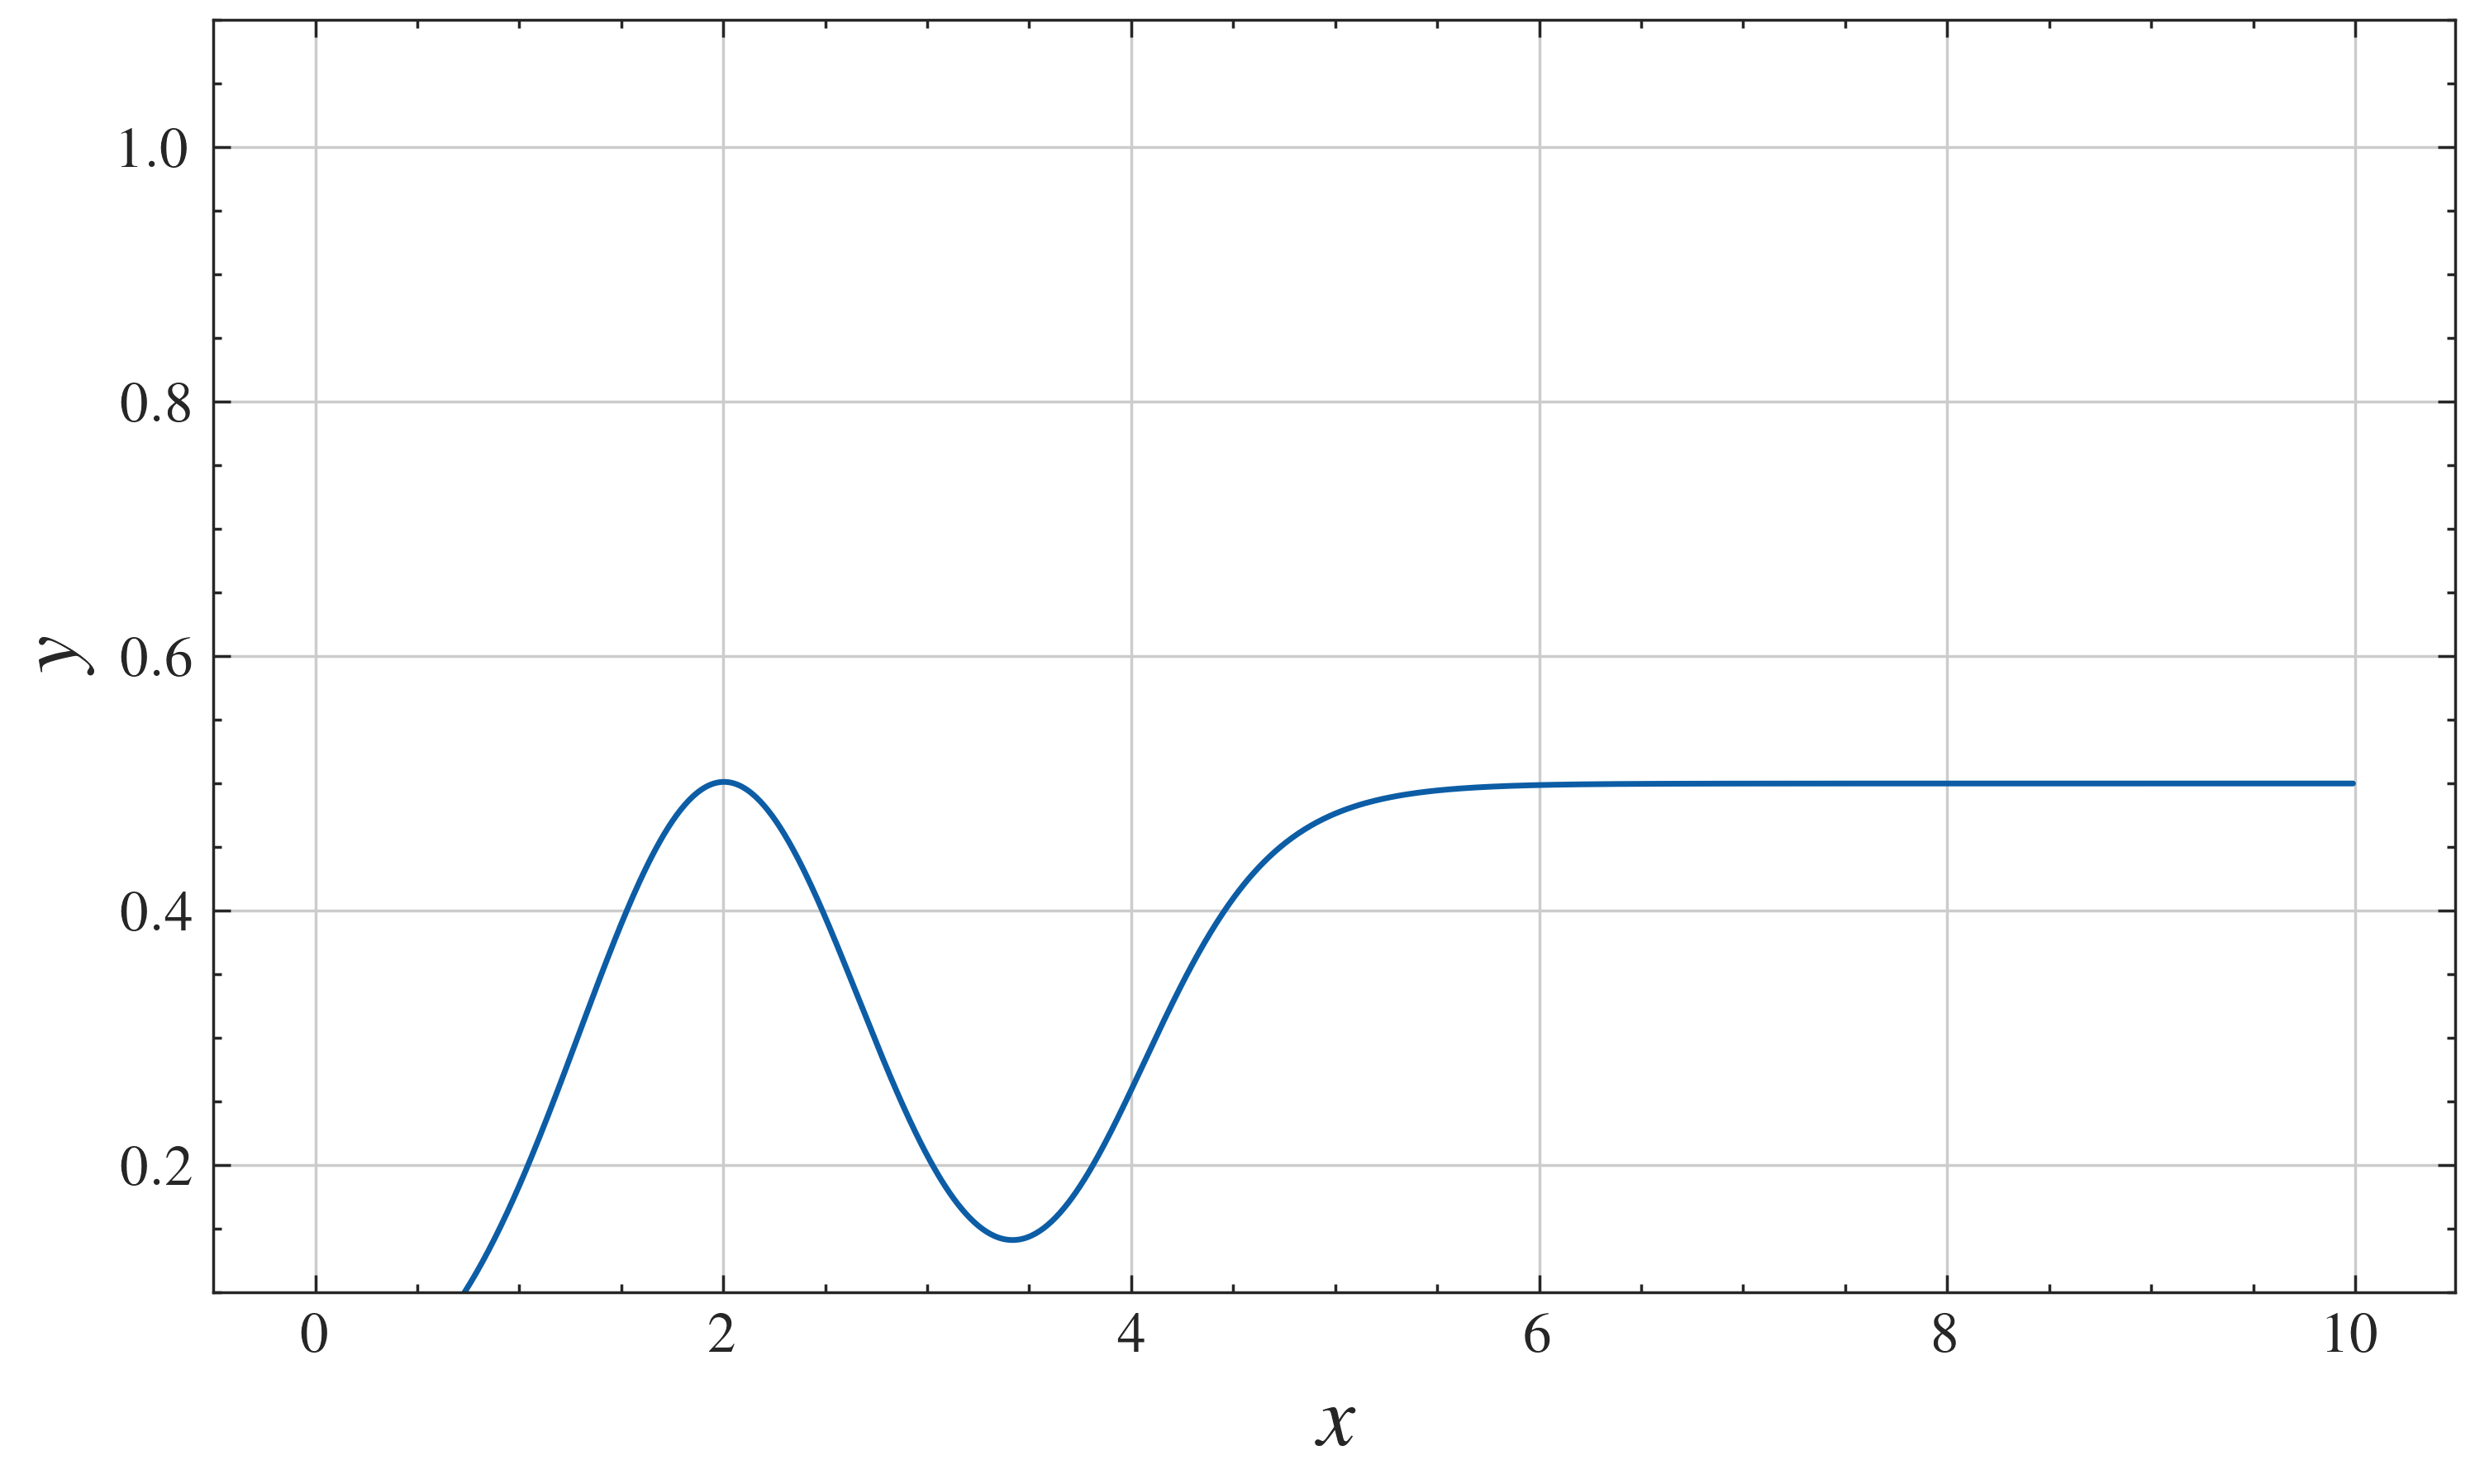
\includegraphics[width=0.8\textwidth]{figures/gaussian_sigmoid.png}
    \caption{\textsc{Activation function $\Phi_{v}$} - \textit{Parameters $\beta=10$, $\alpha=1$, $\mu=1$, $\sigma=1$, and $r=0.5$.}}
    \label{fig:gau_sigm}
\end{figure}


\subsection{Evolution search}
The optimization was carried out over several parameters concerning the model architecture and dynamics:

\noindent \textbf{Network parameters}
\begin{itemize}
    \item $\tau_{u}$: time constant of population $U$
    \item $\tau_{v}$: time constant of population $V$
    \item $g_{u}$: gain of the neural response function of population $U$
    \item $g_{v}$: gain of the neural response function of population $V$
    \item $o_{u}$: offset of the neural response function of population $U$
    \item $o_{v}$: offset of the neural response function of population $V$
    \item $\theta_{u}$: threshold of the neural response function of population $U$
    \item $\theta_{v}$: threshold of the neural response function of population $V$
    \item $W^{+}$: maximal weight value for the weights $\textbf{W}^{UV}$
\end{itemize}

\noindent \textbf{Option value function parameters}
\begin{itemize}
    \item $\beta_{v}$: steepness of the sigmoid
    \item $\alpha_{v}$: shift of the sigmoid
    \item $\mu_{v}$: mean of the Gaussian
    \item $\sigma_{v}$: variance of the Gaussian
    \item $r_{v}$: weight of the sigmoid
\end{itemize}

\noindent \textbf{Learning rate function parameters}
\begin{itemize}
    \item $\beta_{\eta}$: steepness of the sigmoid
    \item $\alpha_{\eta}$: shift of the sigmoid
    \item $\mu_{\eta}$: mean of the Gaussian
    \item $\sigma_{\eta}$: variance of the Gaussian
    \item $r_{\eta}$: weight of the sigmoid
\end{itemize}

\noindent Each individual has been evaluated over environment the following environments:

\begin{itemize}
    \item \textsc{MAB-0}: average reward distribution entropy $\langle H\rangle=2.05$
    \item \textsc{KAB-$\sin$P}: average reward distribution entropy $\langle H\rangle=2.1$, given $K$ arm frequencies $f_{k}$ as an equally spaced set $\{0.1\ldots i\ldots 0.4\}$, phases $\lambda_{k}$ drawn from an uniform $\sim \mathcal{U}(0, 2\pi)$, and half of the arms have been set to constant values drawn from
        another uniform $\sim \mathcal{U}(0.1, 0.7)$; the final reward distribution was not normalized.
\end{itemize}

\noindent The number of arms was $K=10$ and $150$, and lasted for $2$ trials with $2000$ rounds each.
The final fitenss was the average over $2$ iterations.

\hfill \break
The optimization has been implemented in Python using the \texttt{DEAP} library, and the algorithm used was the \texttt{CMA-ES} algorithm. The optimization involved $40$ generations with a population size of $256$ individuals. The mutation rate was set to $0.5$ with a sigma of $0.8$, the cross-over rate was set to $0.4$.
The run were carried out on a 256-core AMD EPYC 7763 with 2TB of RAM.


\subsection{Reward distribution entropy}\label{sec:appendix_entropy}

\noindent The calculation of a set of $N$ reward probability distribution $\mathbf{p}_{i}\text{  for  } i\ldots N$ for $K$ values with a progressively decreasing levels of entropy $\mathbf{h}_{i}\text{  for  } i\ldots N$ has been obtained by the following algorithm:

\begin{algorithm}[ht]
\caption{Reward Probability Distribution Generation}
\label{alg:reward_distribution}
\SetAlgoLined
\KwIn{Number of distributions $N$, dimension $K$}
\KwOut{Set of probability distributions ${\mathbf{p}_i}$ with decreasing entropy}
\SetKwComment{Comment}{// }{ }
\textbf{Initial Setup:}
Define set $B = \{1.5^x \mid x = 1, \ldots, 7\}$; \\
\For{$i \gets 1$ to $N$}{
$\mathbf{z} \gets \text{RandomVector}(0,1)^K$;\\
$j \gets \text{RandomIndex}(K)$;\\
$\mathbf{z}_j \gets 1$;\\
$\beta_i \gets \text{Sample index=} i \text{ from }(B)$ \Comment*[r]{Sample temperature from $B$}

$\mathbf{p}_i \gets \frac{\exp(\beta_i \mathbf{z})}{\sum_j \exp(\beta_i \mathbf{z}_j)}$ \Comment*[r]{Softmax with temperature}
}
\Return ${\mathbf{p}_i}$
\end{algorithm}


\subsection{Table of results}

\textit{\textbf{Note:} table to update}


% weight update over rounds
\subsection{Weight update dynamics}
\noindent We also analyzed the weight update dynamics of the model over the rounds.
In figure \ref{fig:rew_update}, we plotted the evolution of the total weight $\Delta W^{UV}$ over time, averaged over 20 simulations and smoothed over 30 rounds.
The results show that the model is able to quickly adapt to new reward distributions. It is also able to maintain the optimal policy over time, with the weights remaining approximately stable.
The update quantity $\Delta W_{k}^{UV}$, which at each round is applied to one connection $k$, changes sign according to the collected reward, with its magnitude being higher at the beginning of the trials.
Initially, the sign is mostly positive (potentiation) since the weights start at zero, and after some uncertainty a consistently preferred arm emerges.
However, when the reward distribution switches a regular series of sub-optimal choices with respect to the new distribution is made, leading to zero reward.
This causes an accumulation of weight updates with negative sign (depression), eventually bringing the value of the preferred arm to drop. In the meantime, other options are probed until another sequence of choices converges to another arm, promoted by a trail of positive weight updates.

This behaviour is consistent with the low entropy levels observed in the previous analysis.


\begin{figure}[H]
    \centering
    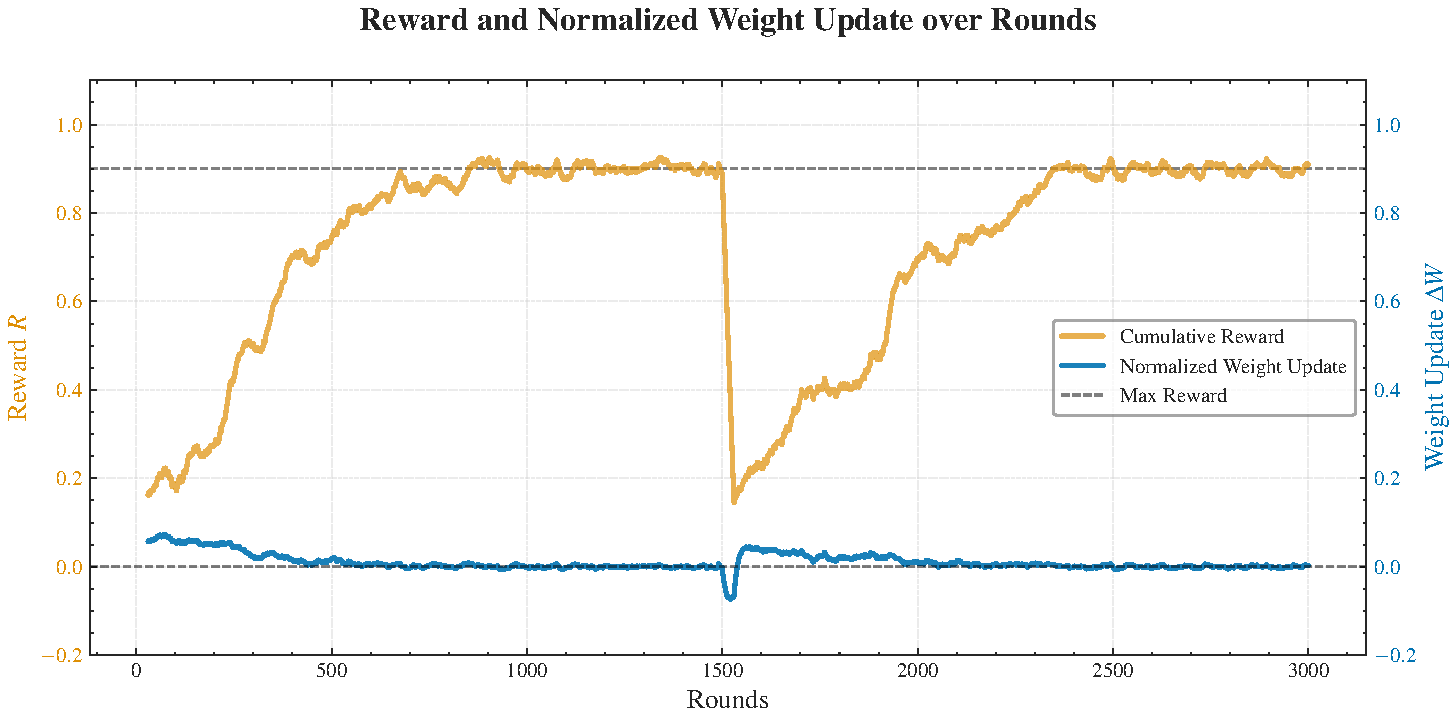
\includegraphics[width=1.0\textwidth]{figures/reward_update_plot.pdf}
    \caption{\textsc{Weight update developement for the model} \textit{The plot displays the weight update quantity $\Delta W_{k}^{UV}$ for each round (blue line), smoothed as a 20-steps moving average.
    It is also reported the average reward in a window of 30 rounds (orange line). The results have been obtained averaging over 20 iterations.}}
    \label{fig:rew_update}
\end{figure}


% % --- table K.5
% \begin{table}[H]
% \centering
% \caption{Performance comparison for $K=5$}
% \label{tab:k5}
% \begin{tabular}{l c c c}
% \toprule
% \textbf{Model} & \textbf{\textsc{KAB-0}} & \textbf{\textsc{KAB-$\epsilon$}} & \textbf{\textsc{KAB-$\sin$}}\\
% \midrule
% Optimal & $0.900$ & $0.881$ & $0.563$ \\
% Random & $0.330$ & $0.337$ & $0.200$ \\
% \midrule
% Thompson & $0.905$ & $0.617$ & $0.317$ \\
% $\epsilon$-Greedy & $0.797$ & $0.531$ & $0.315$ \\
% UCB & $0.897$ & $0.656$ & $0.319$ \\
% \textbf{Model} & $\mathbf{0.899}$ & $\mathbf{0.663}$ & $\mathbf{0.265}$ \\

% \bottomrule
% \end{tabular}
% \end{table}

% % --- table K.10
% \begin{table}[H]
% \centering
% \caption{Performance comparison for $K=10$}
% \label{tab:k10}
% \begin{tabular}{l c c c}
% \toprule
% \textbf{Model} & \textbf{\textsc{KAB-0}} & \textbf{\textsc{KAB-$\epsilon$}} & \textbf{\textsc{KAB-$\sin$}} \\
% \midrule
% Optimal & $0.900$ & $0.885$ & $0.355$  \\
% Random & $0.247$ & $0.250$ & $0.100$ \\
% \midrule
% Thompson & $0.896$ & $0.648$ & $0.339$ \\

% $\epsilon$-Greedy & $0.611$ & $0.597$ & $0.343$ \\
% UCB & $0.891$ & $0.655$ & $0.358$ \\
% \textbf{Model} & $\mathbf{0.905}$ & $\mathbf{0.668}$ & $\mathbf{0.203}$  \\
% \bottomrule
% \end{tabular}
% \end{table}

% % --- table K.100
% \begin{table}[H]
% \centering
% \caption{Performance comparison for $K=100$}
% \label{tab:k100}
% \begin{tabular}{l c c c}
% \toprule
% \textbf{Model} & \textbf{\textsc{KAB-0}} & \textbf{\textsc{KAB-$\epsilon$}} & \textbf{\textsc{KAB-$\sin$}} \\
% \midrule
% Optimal & $0.900$ & $0.883$ & $0.020$  \\
% Random & $0.196$ & $0.201$ & $0.010$ \\
% \midrule
% Thompson & $0.894$ & $0.586$ & $0.013$ \\
% $\epsilon$-Greedy & $0.519$ & $0.574$ & $0.018$ \\
% UCB & $0.853$ & $0.572$ & $0.012$ \\
% \textbf{Model} & $\mathbf{0.898}$ & $\mathbf{0.651}$ & $\mathbf{0.010}$  \\
% \bottomrule
% \end{tabular}
% \end{table}

% % --- table K.200
% \begin{table}[H]
% \centering
% \caption{Performance comparison for $K=100$}
% \label{tab:k200}
% \begin{tabular}{l c c c}
% \toprule
% \textbf{Model} & \textbf{\textsc{KAB-0}} & \textbf{\textsc{KAB-$\epsilon$}} & \textbf{\textsc{KAB-$\sin$}} \\
% \midrule
% Optimal & $0.900$ & $0.885$ & $0.010$  \\
% Random & $0.178$ & $0.176$ & $0.005$ \\
% \midrule
% Thompson & $0.875$ & $0.624$ & $0.006$ \\
% $\epsilon$-Greedy & $0.679$ & $0.588$ & $0.010$ \\
% UCB & $0.792$ & $0.510$ & $0.006$ \\
% \textbf{Model} & $\mathbf{0.905}$ & $\mathbf{0.610}$ & $\mathbf{0.006}$  \\
% \bottomrule
% \end{tabular}
% \end{table}

% % --- table K.1000
% \begin{table}[H]
% \centering
% \caption{Performance comparison for $K=100$}
% \label{tab:k1000}
% \begin{tabular}{l c c c}
% \toprule
% \textbf{Model} & \textbf{\textsc{KAB-0}} & \textbf{\textsc{KAB-$\epsilon$}} & \textbf{\textsc{KAB-$\sin$}} \\
% \midrule
% Optimal & $0.900$ & $0.880$ & $0.002$  \\
% Random & $0.177$ & $0.178$ & $0.001$ \\
% \midrule
% Thompson & $0.779$ & $0.445$ & $0.001$ \\
% $\epsilon$-Greedy & $0.386$ & $0.478$ & $0.002$ \\
% UCB & $0.301$ & $0.185$ & $0.001$ \\
% \textbf{Model} & $\mathbf{0.703}$ & $\mathbf{0.480}$ & $\mathbf{0.001}$  \\
% \bottomrule
% \end{tabular}
% \end{table}


% \newpage
